%! alt Triangle ABC with BC = 7, CA = 20 and AB = 15, and its circumcircle with centre O. The foot H of the altitude from A lies on line BC beyond B, so the angle at B is obtuse. Segment AO is parallel to BC and so perpendicular to the altitude AH, and angle B exceeds angle C by 90 degrees.
%! after_paragraph 1
%! scale 1/3.2
% The shared preamble of every Cevian figure. pipeline/figures turns these colours into theme-aware paint,
% and refuses any other colour, so draw only with them:
%   figink (lines and labels), figaux (construction lines), figaccent (the object the argument turns on),
%   figtint and figaccenttint (light fills).
\documentclass[border=1.5pt]{standalone}
\usepackage{tkz-euclide}
\definecolor{figink}{RGB}{0,0,0}
\definecolor{figaux}{RGB}{85,85,85}
\definecolor{figaccent}{RGB}{192,57,43}
\definecolor{figtint}{RGB}{221,221,221}
\definecolor{figaccenttint}{RGB}{245,213,208}
% tkz-euclide's defaults draw circles, compasses and marks in 50% grey and fill points with a tint.
\makeatletter
\def\tkz@otherlinecolor{figink}
\def\tkz@euc@circlecolor{figink}
\def\tkz@euc@compasscolor{figink}
\def\tkz@euc@mkcolor{figink}
\def\tkz@mk@fill{figink}
\def\tkz@euc@pointfillcolor{figink}
\makeatother
\tkzSetUpLine[color=figink,line width=.7pt]
\tkzSetUpArc[color=figink,line width=.7pt]
\tkzSetUpCompass[color=figink,line width=.5pt]
\tkzSetUpPoint[color=figink,fill=figink,size=3.1pt]
\tikzset{
  every picture/.style={line cap=round,line join=round,color=figink},
  circle style/.append style={color=figink,line width=.7pt},
  aux/.style={color=figaux,line width=.45pt,dash pattern=on 2.6pt off 2pt},
  key/.style={color=figaccent,line width=1pt},
  mk/.style={color=figink,line width=.5pt},
  lbl/.style={color=figink,inner sep=2.2pt},
  len/.style={color=figink,inner sep=1.5pt,font=\small},
}

\begin{document}
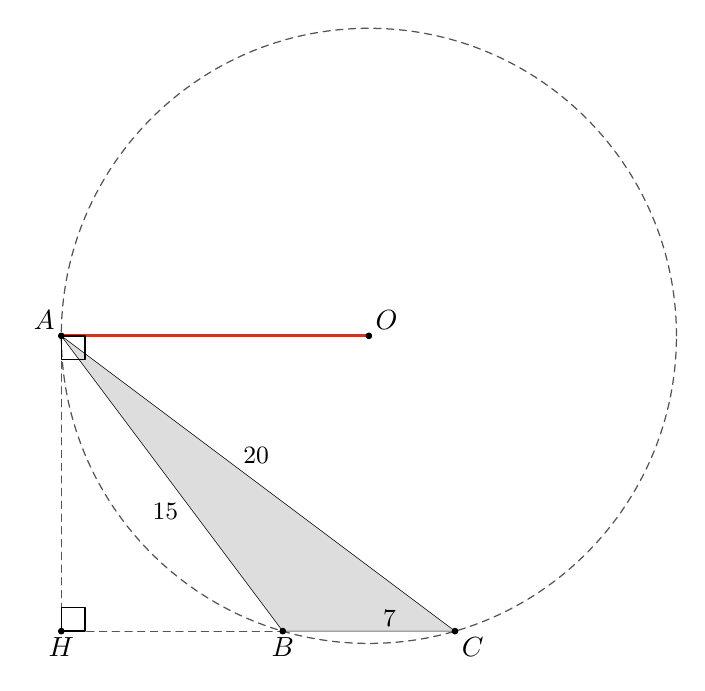
\begin{tikzpicture}
\tkzDefPoint(0.0,0.0){B} %! B = (0, 0)
\tkzDefPoint(2.1875000,0.0){C} %! C = (7, 0)
\tkzDefPoint(-2.8125000,3.7500000){A} %! A = (-9, 12)
\tkzDefPoint(1.0937500,3.7500000){O} %! O = (7/2, 12)
\tkzDefPoint(-2.8125000,0.0){H} %! H = foot(A, B, C)
%! fact parallel(O, A, B, C)
%! fact perp(A, H, B, C)
%! fact perp(A, H, A, O)
%! fact dist(O, A) == dist(O, B)
%! fact dist(O, C) == dist(O, B)
%! fact angle(A, B, C) - angle(A, C, B) == 90
%! example dist(B, C) == 7
%! example dist(C, A) == 20
%! example dist(A, B) == 15
\tkzDrawCircle[aux](O,B)
\tkzFillPolygon[color=figtint](A,B,C)
\tkzDrawSegment[aux](H,B)
\tkzDrawSegment[aux](A,H)
\tkzDrawPolygon(A,B,C)
\tkzDrawSegment[key](A,O)
\tkzMarkRightAngle[size=.3,mk](B,H,A)
\tkzMarkRightAngle[size=.3,mk](H,A,O)
\tkzDrawPoints(A,B,C,O,H)
\tkzLabelPoint[above left,lbl](A){$A$}
\tkzLabelPoint[below,lbl](B){$B$}
\tkzLabelPoint[below right,lbl](C){$C$}
\tkzLabelPoint[above right,lbl](O){$O$}
\tkzLabelPoint[below,lbl](H){$H$}
\tkzLabelSegment[above,pos=.62,len](B,C){$7$}
\tkzLabelSegment[above right,pos=.45,len](A,C){$20$}
\tkzLabelSegment[below left,pos=.55,len](A,B){$15$}
\end{tikzpicture}
\end{document}
